\chapter{Analisa Sistem Tak Ubah Waktu}

\section{Pengantar}
Sinyal dan sistem merupakan sebuah kesatuan yang saling berhubungan satu sama lain. Sinyal merupakan pola-pola bervariasi yang berubah terhadap satu atau lebih variabel bebas, yang berisi informasi tentang perilaku atau sifat dari suatu fenomena tertentu. Sistem akan menerima sinyal untuk kemudian mengelola, mengolahnya sehingga menhasilkan keluaran atau tanggapan berupa sinyal lain ataupun perilaku atau sifat tertentu sesuai keinginan. Penerapan sinyal dan sistem ada dalam banyak bidang yang bervariasi mulai dari teknologi komunikasi, elektronika, komputer, pembangkit energi, pengolahan suara untuk musik, transportasi, sampai kendali otomatis pada proses-proses di industri. Masih banyak lagi penerapan sinyal dan sistem dalam kehidupan sehari-hari yang kita sadari atau tidak telah kita gunakan secara rutin dalam kehidupan kita. Penerapan-penerapan tersebut kesemuanya memiliki pola dan ciri mendasar seperti yang telah dijabarkan pada awal paragraf. Contoh sederhananya adalah mobil. Mobil bergerak dan melaju dengan kecepatan tertentu akibat adanya injakan dari pedal gas, dalam hal ini injakan pada pedal gas merupakan sinyal masukan bagi sistem mobil dan sistem mobil melalui proses mekanis dan termodinamik pada mesinnya akan menhasilkan tanggapan berupa laju mobil yang sesuai dengan seberapa dalam injakan pedal gas. Contoh lain terdapat pada rangkaian listrik, dimana sinyal masukan berupa arus dan tegangan listrik yang berubah terhadap waktu pada sistem rangkaian listrik yang dapat berupa komponen-komponen elektronik dan elektrik seperi resistor, kapasitor dan lain-lain akan menghasilkan tanggapan berupa arus dan tegangan yang berbeda sesuai dengan yang diinginkan. 

\begin{figure}[!h]
\centering
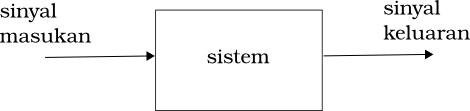
\includegraphics[scale=0.7]{pict/sinyalsistem}
\caption{Representasi konsep sinyal dan sistem dalam diagram blok}\label{sinyalsistem}
\end{figure}

Konsep sinyal dan sistem muncul dalam dalam berbagai aplikasi yang berbeda bergantung pada bagaimana pengunaan konsep tersebut. Konsep sinyal dan sistem dapat digunakan untuk mengkaraterisasi sebuah sistem. Mengkarakterisasi berarti membaca karakter atau sifat dari sebuah sistem tertentu dengan cara memberikan sinyal masukan yang bervariasi dan membaca bagaimana sistem menanggapai masukan yang bervariasi tersebut. Hal ini seperti apabila kita mempunyai sebuah kotak hitam yang kita tidak tahu sepeti apa sifat dan bagaimana kotak hitam tersebut bekerja. Dengan memberikan masukan bervariasi terhadap kotak hitam tersebut maka akan dapat diperoleh keluaran barupa tanggapan yang berbeda dengan masukan, sehingga dengan ini kita dapat mengetahui apa dan bagaimana kotak hitam misterius ini berperilaku atau bekerja. Konsep sinyal dan sistem juga dapat digunakan untuk melakukan pemrosesan terhadap sinyal tertentu agar diperoleh keluaran sinyal sesuai yang diharapkan atau untuk menghilangkan sinyal yang tidak diinginkan. Contohnya adalah dalam sistem \textit{noise canceling} (NC) atau pembatal bising. Dalam sistem NC yang biasa digunakan pada speaker, bising atau suara mengganggu yang tidak diinginkan dari dapat diredam sedemikian hinga sehingga suara atau bunyi yang keluar dari \textit{speaker} adalah ahanya suara yang diharapkan. Sistem NC akan membangkitkan suara dengan frekuensi tertentu yang sama dengan suara bising tertentu tetapai dengan fase yang berbeda sehingga melalui proses interferensi suara bising dapat diredam. 

